\chapter{The Logging Mechanism of Dresden OCL}
\label{chapter:logging}

\begin{flushright}
\textit{Chapter written by Claas Wilke}
\end{flushright}

Dresden OCL uses a \keyword{Log4j Logger} to log method entries, exits and
errors during Dresden OCL's execution. Each plug-in of Dresden OCL provides a
\code{log4j.properties} file that can be used to configure the logger for the
plug-in. Listing~\ref{logging:lst:log4j} shows such file of the Model Bus
plug-in.

\begin{figure}[!t]
  \lstset{language=XML,keywords={}}
  \lstinputlisting[caption={The
  Log4J configuration of the ModelBus
  plug-in.},label={logging:lst:log4j}]{figures/logging/log4j.properties}
\end{figure}

The last line of this configuration file (line 25) configures the logger. You
can configure the logger to log messages of three different levels
(\code{info}, \code{debug} and \code{error}). Furthermore, you can use different
appenders to collect the logging messages such as the console (\code{stdout}) or
an socket-based logging service (\code{socket}). The standard configuration of
Dresden OCL's plug-ins is to log only error messages using the \code{stdout}
appender.

If you use the \code{socket} appender instead, you might
receive exceptions on the console like the following, although the toolkit 
works correctly.

\begin{center}
\reference{log4j:ERROR Could not connect to remote log4j server at [localhost].}
\end{center}

The reason is that the Log4j Logger tries to sent the logged events to a server 
running at \url{localhost}. To solve this problem (if you want to) you have to 
install and setup a logging server at your computer. One logging server you
might use is called \keyword{Chainsaw} and available at the Apache Logging 
website \cite{WWW:chainsaw}. If you start Chainsaw, set up a 
\keyword{SocketReceiver} at port \keyword{4445 (Old Style/Standard Chainsaw 
Port)} (cf. Figure~\ref{pic:logging:chainsaw01}). Afterwards, the logging error 
message should not occur anymore.

\begin{figure}[!htbp]
	\centering
	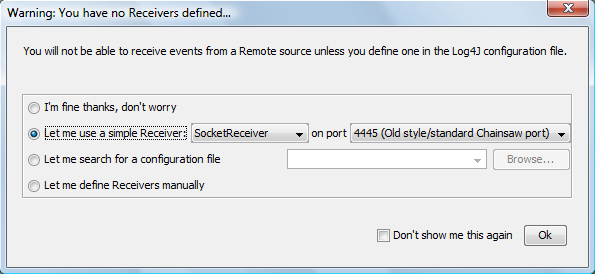
\includegraphics[width=0.8\linewidth]{figures/logging/chainsaw01}
	\caption{Setting up a simple SocketReceiver in Chainsaw.}
	\label{pic:logging:chainsaw01}
\end{figure}